\chapter{Evaluation}
\label{cha:evaluation}

We need to describe here some details about how did we evaluate that our graph is correct e.g. show-casing screens from user interface or QGIS etc. Then we need to show how did we test our code, if it scales, and maybe some performance measurements

\section{Clustering algorithm}

In this section we will describe how we evaluated our dbscan algorithm and the choice of the \textit{epsilon} and \textit{minimum points per cluster} parameter.

\subsection{DBSCAN}

We visualised our results in QGIS, a powerful graph visualisation tool. Running the dbscan with different parameters resulted in different cluster sizes and number of clusters. We started off with the target area of Berlin. The \textit{epsilon} parameter (radius of the cluster) was chosen by looking at the graininess (accuracy) of our given data set. The accuracy between points was 110 meters, this distance is refered to as \textit{accuracy distance}.
We took Alexanderplatz in Berlin as an example cluster (a popular train stop area in Berlin). We interpret one cluster as being one stop point of interest, and for this application want Alexanderplatz to be represented as one cluster. Setting the \textit{epsilon} parameter to the \textit{accuracy distance},  110 meters, gave us good looking clusters whilst higher value of the parameter resulted in clusters being unnaturally large and distance below the \textit{accuracy distance} resulted in only single-point clusters (points are stacked at the same location). Note that the \textit{minPts}, minimum points per cluster, parameter is not taken into \textit{consideration} here (it is set arbitary and only determines the number of clusters, while we here are interested in the \textit{size} of the clusters). See figures below.

 
\begin{figure}[!ht]
	\centering
	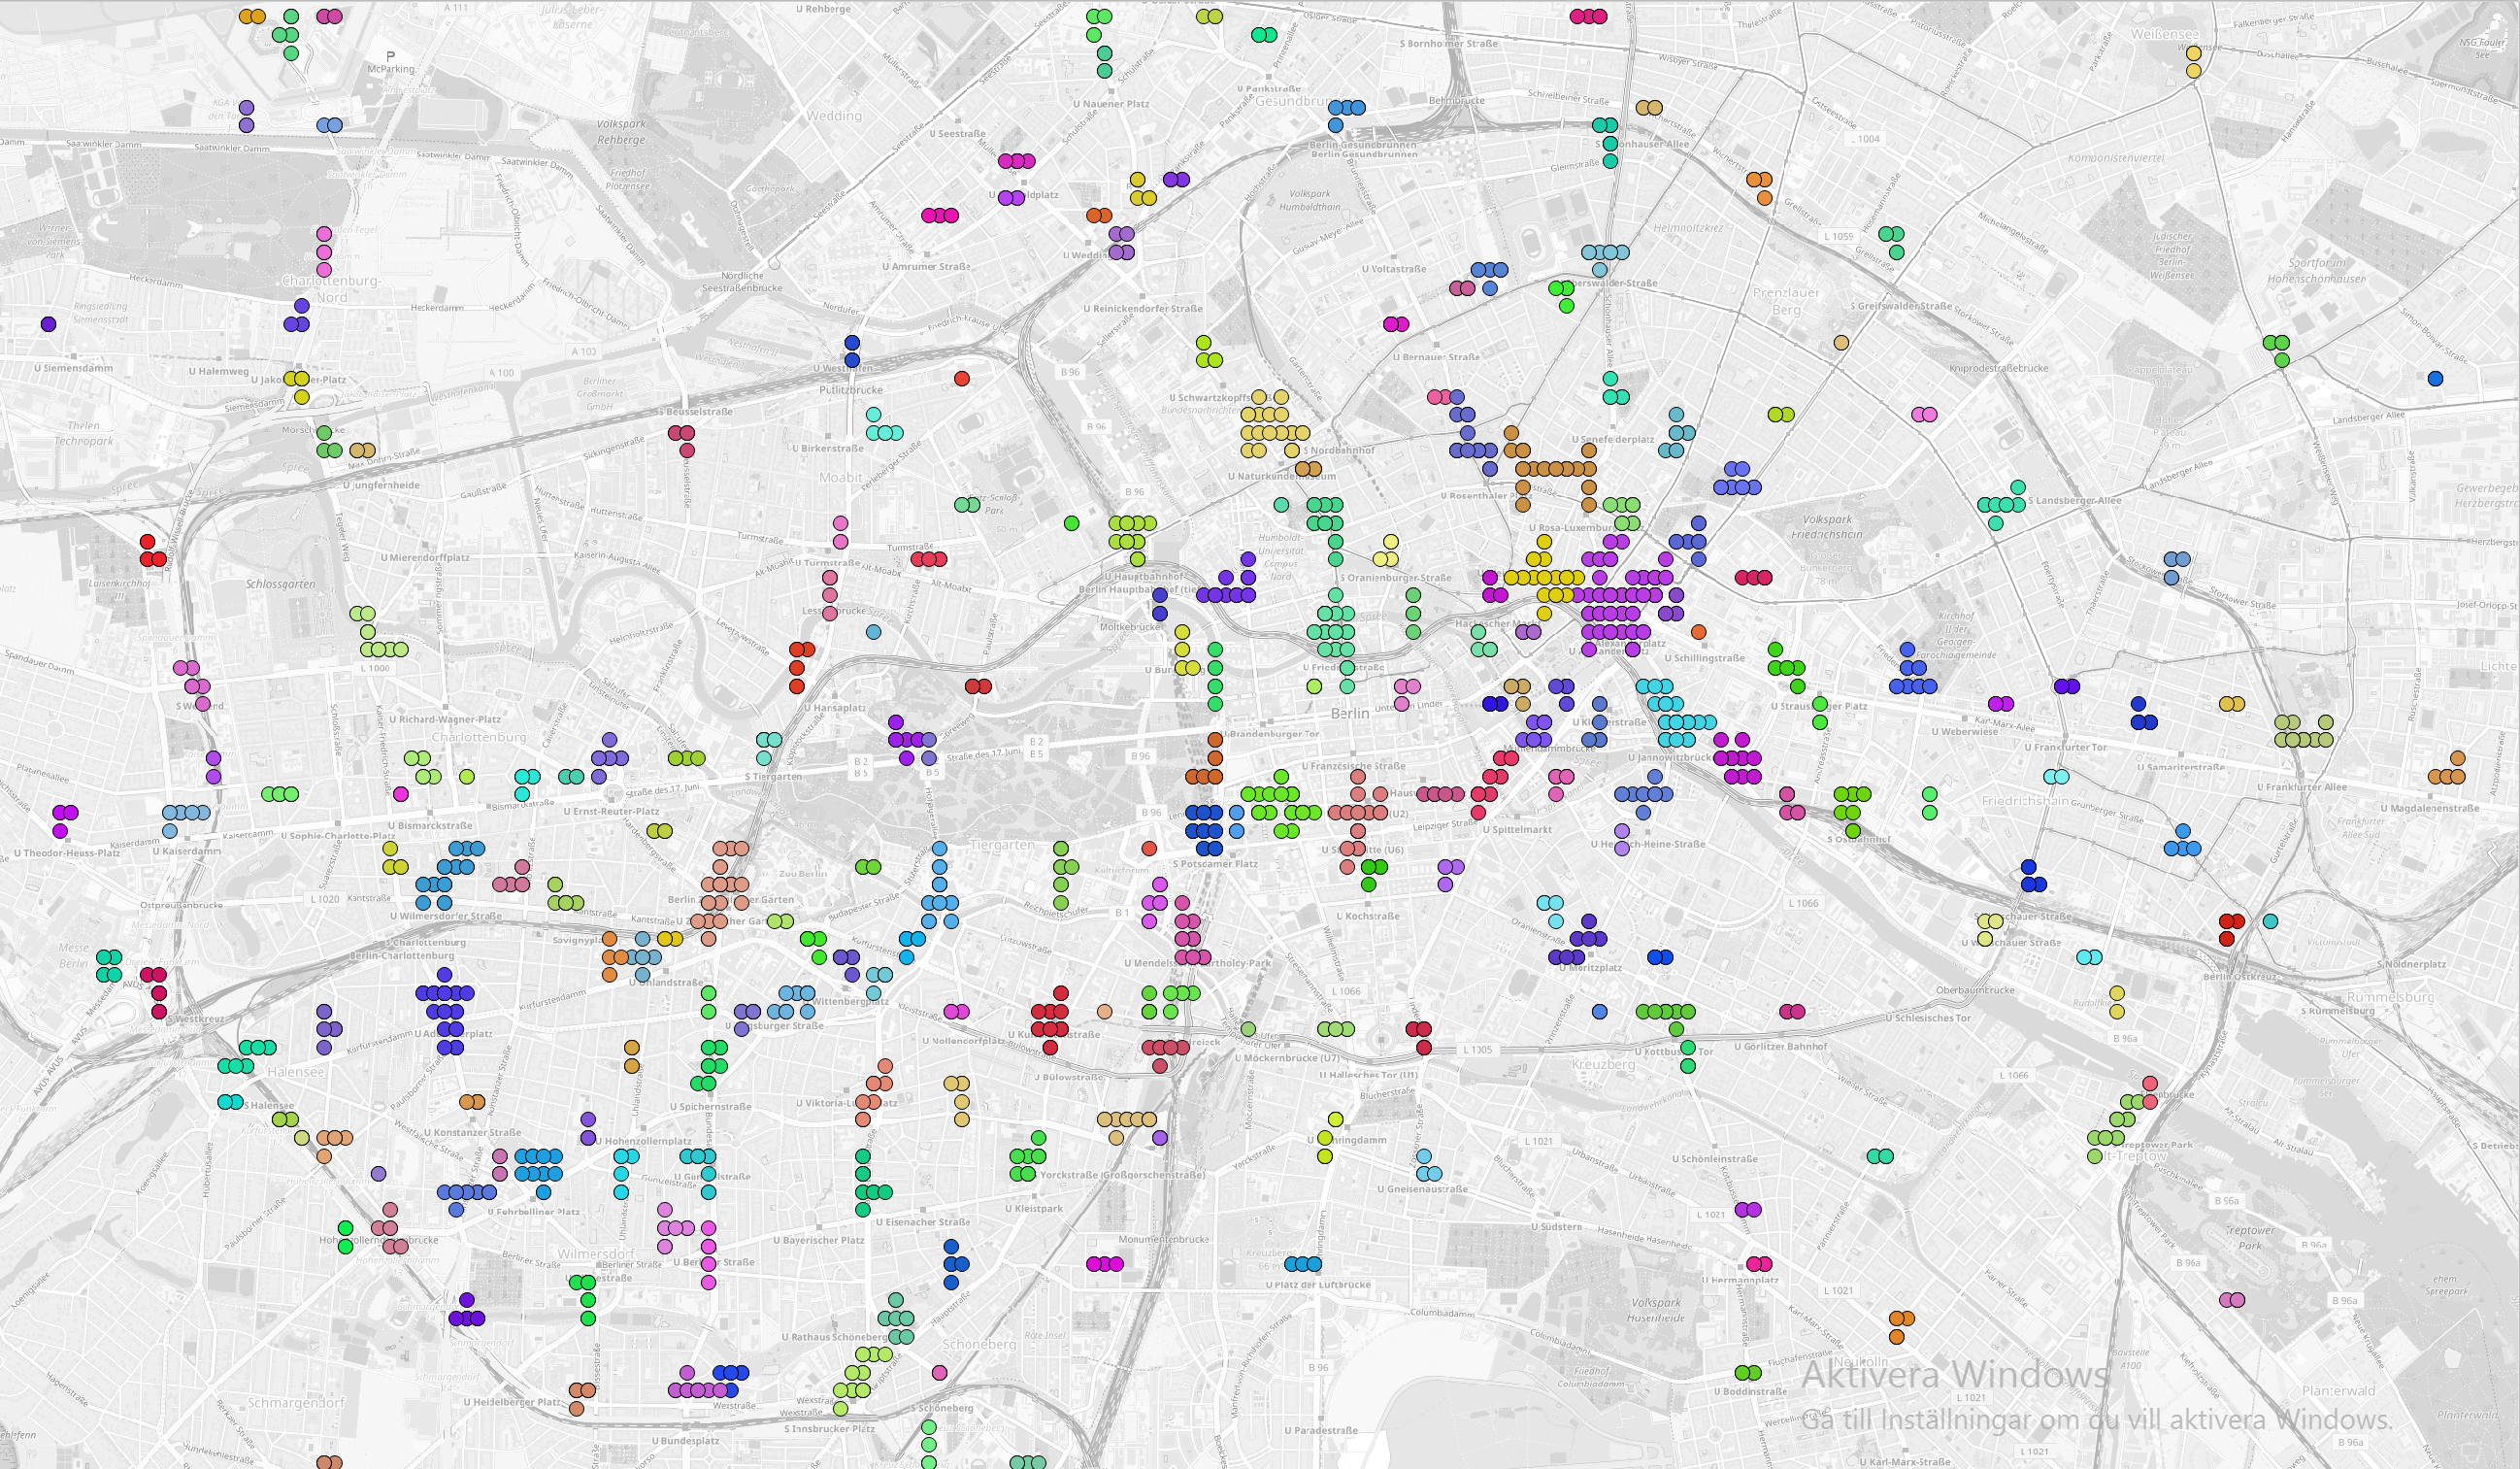
\includegraphics[width=1\textwidth]{images/0,001_5_gray.png}\\
	\caption{ Clusters with good parameters \textit{epsilon} = 110 meter, \textit{minPts} = 5. Alexanderplatz (pink) has 85 data points in it.  }
	\label{fig:0.001_5_gray}
\end{figure}

\begin{figure}[!ht]
	\centering
	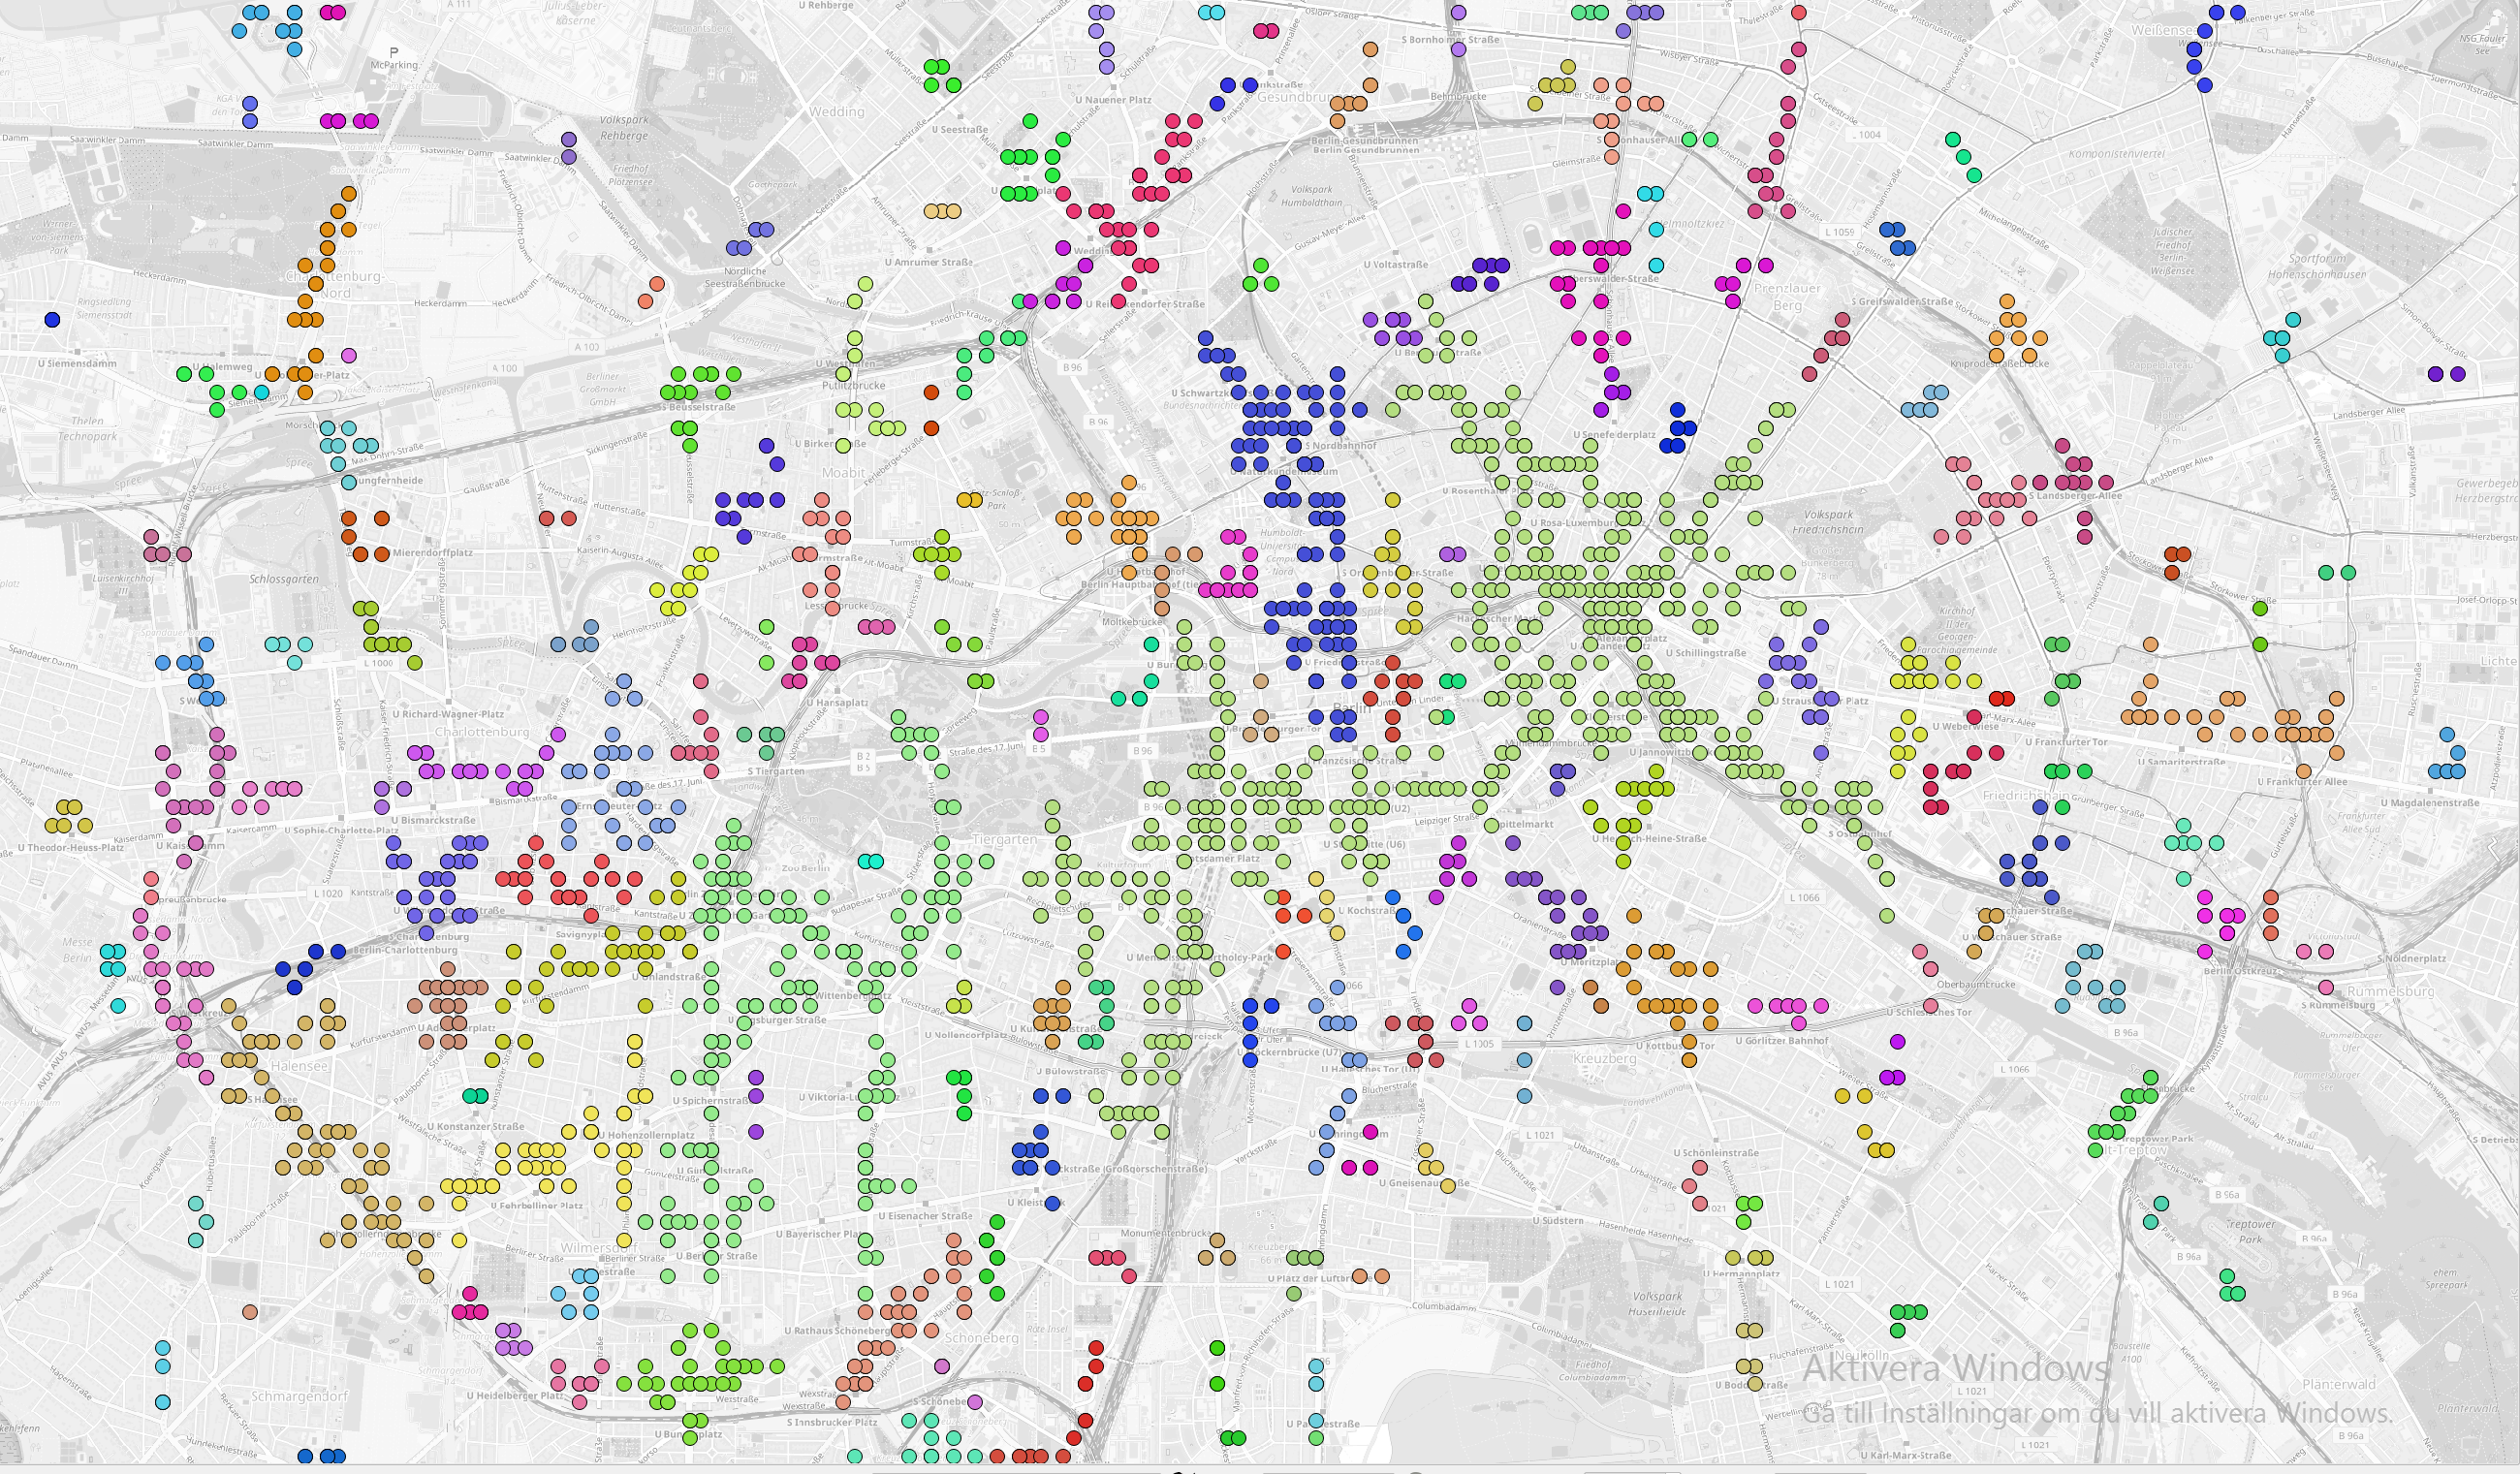
\includegraphics[width=1\textwidth]{images/0,002_5_gray.png}\\
	\caption{ Example of a clusters with bad parameters, here \textit{epsilon} = 220 meter is too large, \textit{minPts} = 5. "Alexanderplatz" (light green) has 748 data points in it and stretches over the whole centre (Mitte) of Berlin. }
	\label{fig:002_5_gray}
\end{figure}
 

